\begin{titlepage}
    \begin{tikzpicture}[overlay,remember picture,line width=5pt]
        \node[inner sep=0pt] at ($(current page.center)+(0,3)$) {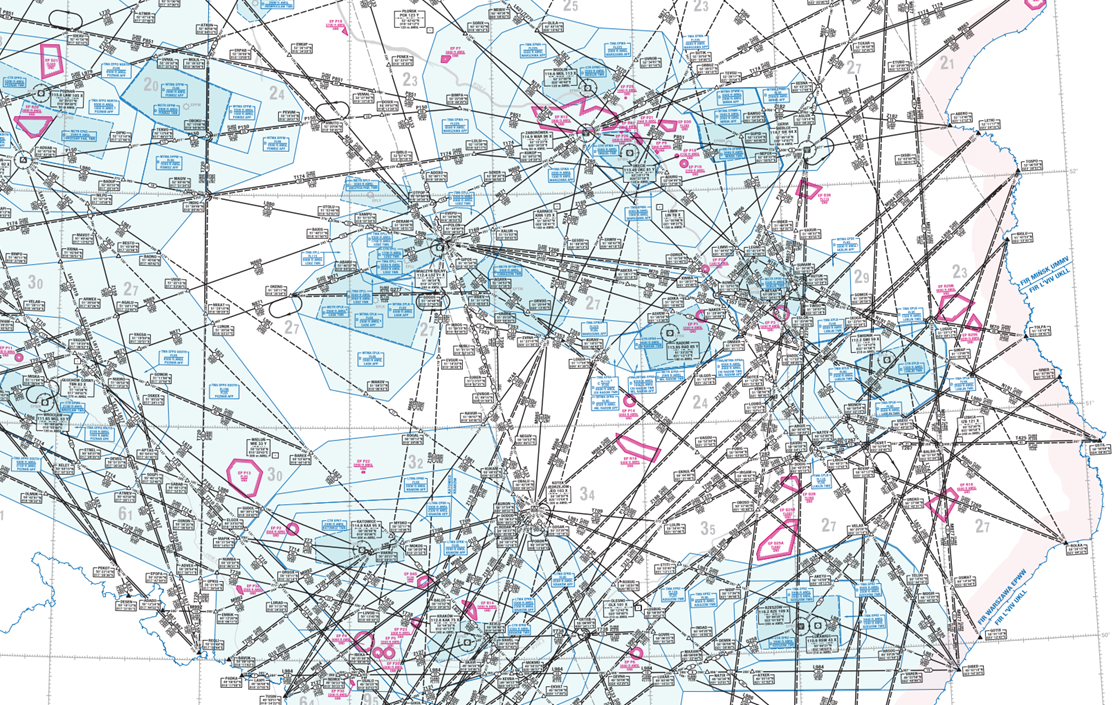
\includegraphics{bg/map.png}};
        \path[fill=white, drop shadow={opacity=0.25}] (current page.north west)--($(current page.north west)+(0,-3)$)--($(current page.north)+(0,-5)$)--($(current page.north east)+(0,-3)$)--(current page.north east)--cycle;
        \node[inner sep=0pt] at ($(current page.north)+(0,-2)$) {
\includegraphics[width=15cm]{logo.png}};
        \path[fill=vred!75!black] ($(current page.south west)+(0,13)$) -- ($(current page.south east)+(0,10)$) -- (current page.south east) -- (current page.south west) -- cycle;
        \path[fill=vred, drop shadow={opacity=0.25}] (current page.south west) -- ($(current page.south west)+(0,8)$) -- ($(current page.south east)+(0,15)$) -- (current page.south east) -- cycle;

        \node[inner sep=0pt] at ($(current page.south west)+(4,3)$) {
\includegraphics[width=5cm]{vatsim.png}};
        \node[inner sep=0pt] at ($(current page.south east)+(-4,3)$) {
\includegraphics[width=5cm]{vateud.png}};
        \node(title) at ($(current page.center)+(0,-8)$) {\color{white}{\textbf{\Huge{OPERATIONS MANUAL}}}};
        \node(subtit) at ($(title)+(0,-2)$) {\color{white}{\Huge{vFIR Warszawa}}};
        \node(rev) at ($(current page.south)+(0,2)$) {\color{white}{Revision \revision}};
    \end{tikzpicture}
\end{titlepage}

\begin{tcolorbox}[
    colback=white,
    %halign=center,
    %halign lower=center,
    %halign title=center,
    colframe=vred,
    enhanced,
    %leftrule=3mm,
    before title={\faExclamationTriangle~},
    title=\LARGE\textbf{Disclaimer}
]
    \textbf{This document is intended for use on VATSIM network only.}
    \tcblower%
    Do not use for training purposes or in real life scenarios.
\end{tcolorbox}